\hoofdstuk{Conclusion and recommendations}

At the start of this thesis the following questions were asked: `How can license plate information be gathered from the images of a smartphone camera using software?', `How can the software be optimized to work in a correct way from within a mobile device?' and `What are the limitations of such an application?'. Using the information gathered during the course of the project, these questions will now be answered.

\paragraaf{How can license plate information be gathered from the images of a smartphone camera using software?}

\paragraaf{How can the software be optimized to work in a correct way from within a mobile device?}

Because smartphones are limited devices when it comes to processing power, when creating such an application these limitations must be taken into account. This was solved using two different approaches: multi-threading and buffers.

Starting with multi-threading, this technique allows an application to share its processing load with every processor core in the smartphone. The application uses four threads for its main four components: the UI thread, the band localization thread, the plate localization thread and the text recognition thread. This allows for, in the case of the smartphone used to test the application, a dedicated core for every thread. Every time there is a new item available in one of the buffers, the respective thread is executed with the new data.

The buffers approach takes into consideration that a smartphone does not have enough processing power to process images at real-time. The outputs of every thread, with the exception of the text recognition thread because its output is handled immediately, are therefore stored within a buffer so they can be processed in their own time. There are 3 different buffers: the frames buffer, the bands buffer, and the plates buffer. 
The frames buffer stores the video frames capture with the smartphone's camera and has a maximum size of 1. This prevents the accumulation of frames which were captured shortly after each other which leads to a high chance of processing the same plate multiple times. The other two buffers store bands and plates respectively and have no size limitations because when the initial frame has been processed, the follow-up data is considered important and is processed evenly.

Using this two methods it's possible to create a functional application despite its need for a large amount of processing power.


\paragraaf{What are the limitations of such an application?}

Because of the nature of this application, it brings a couple of problems to its usability. One of these problems is the distance at which the application can still process a plate reliably. After performing tests to find this maximum distance, the results indicated the application was still able to provide reliable results at the distance of 5 meters, while at the distance of 6 meters it was still able to sometimes provide correct results but not in a reliable manner. The other problem is the angle at which the results are still processed correctly. Tests demonstrated that the maximum angle is located at around 47,5$^{\circ}$ at a distance of 4 meters. Using this information, an area can be derived where the application works well and where it starts having problems. This area is depicted in Figure \ref{fig:road-situation} and the scenario was created using the road design criteria from the province of Zuid-Holland \cite{road-design}. Looking at this figure it's clear that the application can process the plates of vehicles both in the same lane and in the adjacent lanes while driving at a safe distance.

\begin{figure}[ht]
    \centering
    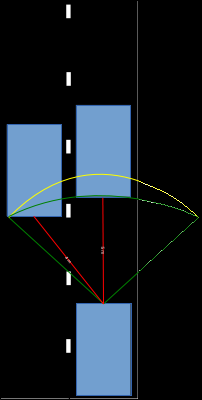
\includegraphics[width=0.3\textwidth]{plaatjes/roadeye-road}
    \caption{Application flow diagram.}
    \label{fig:road-situation}
\end{figure}%
